\section{Quellencodierung}
\subsection{Redundanz}
Anteil in einer Codierung, die keine Information trägt. \\
Mittlere Länge einer Codierung:
\[L= \sum_{n=0}^{N=1} P(x_n)\cdot l_n\]
Redundanz:
\[R=L-H\]
\textbf{Beispiel: Packed BCD, Ziffern 0...9 codiert in 4 Bit}
\begin{enumerate}
    \item $P(x_{0...9}) = 0.1$
    \item Entropie, $H_{BCD} = 10 \cdot 0.1 \cdot \log_{2}{10} = 3.32$ Bit pro Symbol
    \item Code Länge, $L_{BCD} = 4$ Bit pro Symbol
    \item Redundanz, $R = L_{BCD} - H_{BCD} = 4 - 3.32 = 0.68$ Bit pro Symbol
\end{enumerate}

\subsubsection{Kompressionsrate}
Die Kompressionsrate $R$ ist der Quotient von komprimierten Bits durch originale Bits. Obwohl Kompressionsrate und Redundanz beide mit $R$ bezeichnet werden, haben diese Grössen nichts miteinander zu tun.

\subsubsection{Codes unterschiedlicher Länge}
Codes unterschiedlicher Länge sind möglich, Voraussetzung ist jedoch die Präfixfreiheit. D.h. kein Code bildet den Anfang eines anderen Codes.

\subsubsection{Theorem zur Quellencodierung}
\begin{enumerate}
    \item Solange die Redundanz R eines Codes grösser als null ist, kann verliustfrei komprimiert werden.
    \item Falls $R \leq 0$, so kann nur verlustbehaftet komprimiert werden.
\end{enumerate}

\subsection{Lauflängencodierung}
Ketten von identischen Zeichen werden zusammengefasst. RLE codiert runs wie folgt: (Marker, Anzahl, Zeichen)
\begin{enumerate}
    \item Als Marker wird ein selten genutzter Code verwendet. Hier A.
    \item Eine Zählerbreite in Bits wird so gewählt, dass Runs der typischen Länge damit erfasst werden können.
    \item Annahme: 2-Bit-Symbole und 6-Bit-Zähler: M+A+Z = 2+6+2 = 10 Bit.
    \item Beispiel:
    \[\mathtt{TERRRRRRRRRMAUIIIIIIIIIIIIIIIIIWQCSSSSSSSSSSL}=\]
    \[\mathtt{TEA09RMA01AUA17IWQCA10SL}\]
\end{enumerate}

\subsection{Huffman Codes}
\subsubsection{Verfahren}
\begin{enumerate}
    \item Ordne alle Symbole nach aufsteigenen Auftretenswahrscheinlichkeiten auf einer Zeile. Dies sind die Blätter des Huffman-Baums.
    \item Notiere unter jedes Blatt seine Wahrscheinlichkeit.
    \item Schliesse die beiden Blätter mit der kleinsten Wahrscheinlichkeit an einer gemeinsamen Astgabel an und ordne dem Ast die Summe der Wahrscheinlichkeiten der beiden Blätter zu.
    \item Wiederhole Punkt 3 mit Blättern und Ästen so lange, bis nur noch der Stamm des Baums übrig bleibt.
    \item Nun wird bei jeder Astgabel dem einen Zweig eine 0 und dem anderen eine 1 zugeordnet. (Die Zuordnung ist frei wählbar, muss aber über den ganzen Baum einheitlich sein).
    \item Nun werden auf dem Pfad vom Stamm zu jedem Blatt die Nullen und Einsen ausgelesen und von links nach rechts nebeneinander geschrieben. Dies sind die Huffman-Codeworte.
\end{enumerate}
\begin{align*}
    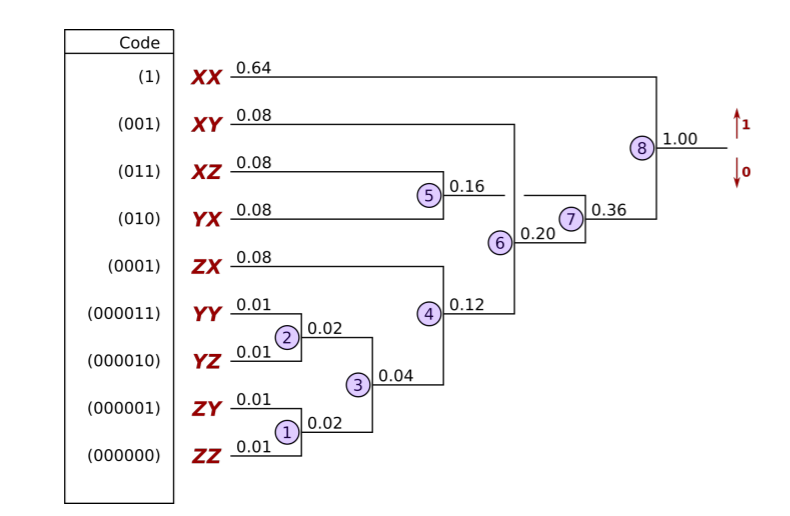
\includegraphics[width=1\linewidth]{images/huffman.png}
\end{align*}

\subsection{LZ77}
Alle Zeichen werden durch Token fixer Länge ersetzt. Token: (Offset, Länge, Zeichen)
\begin{align*}
    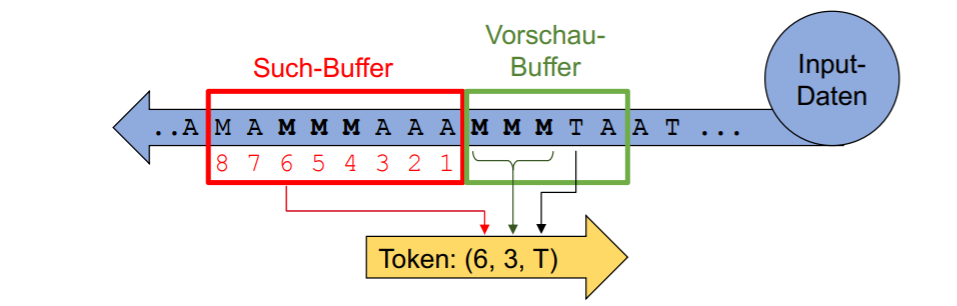
\includegraphics[width=1\linewidth]{images/lz77.png}
\end{align*}

\subsection{LZW}
\begin{enumerate}
    \item Statt einem Sliding Window wird ein Wörterbuch verwendet
    \item Der Index nummeriert die Einträge des Wörterbuchs
    \item Der String bildet den eigentlichen Eintrag
    \item Wörterbuch wird initialisiert mit den möglichen Zeichen resp. Byte-Werten (0..255). à Einzelne Zeichen sind im WB immer vorhanden.
    \item Token enthält nur den Index des schon bestehenden Eintrags im Wörterbuch, nicht aber das zusätzliche Zeichen. Token: (Index)
    \item Das neue Zeichen wird erst mit dem nächsten Token übermittelt (Überlappung)
\end{enumerate}
\textbf{Beispiel: } $\mathtt{A M A M M M A A A M M M T A A T ...}$
\begin{align*}
    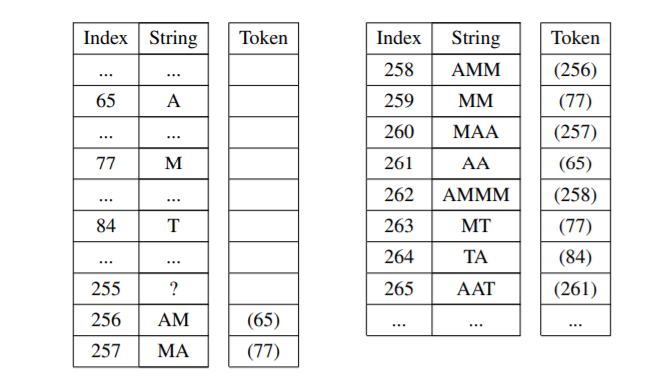
\includegraphics[width=1\linewidth]{images/lzw.png}
\end{align*}

\subsection{Bildkompression - JPEG}

\begin{center}
    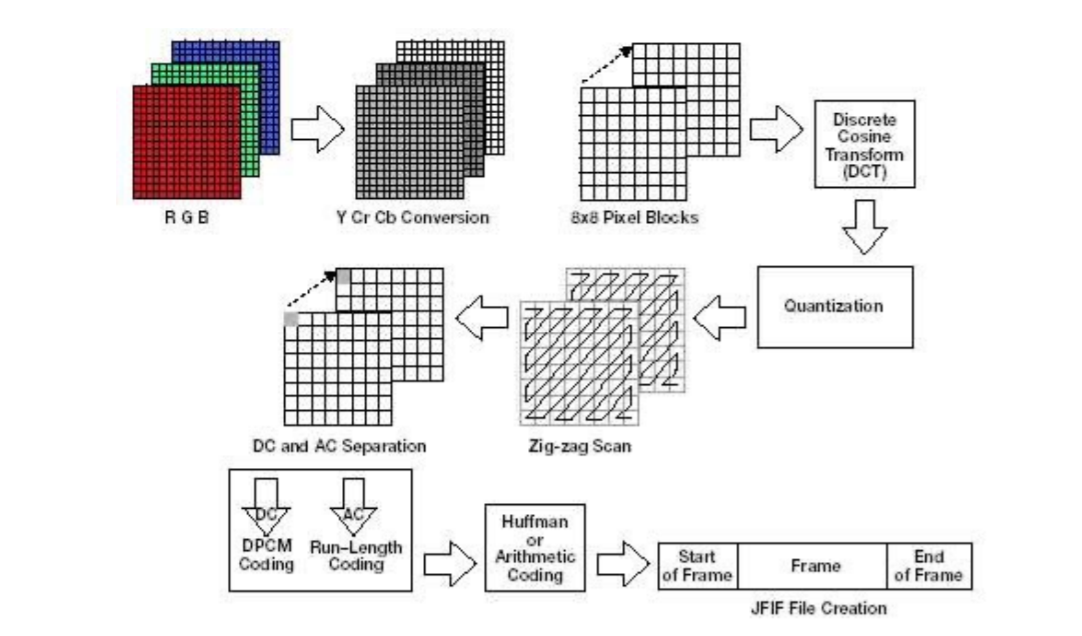
\includegraphics[width=1\linewidth]{images/verfahren.png}
\end{center}

\subsubsection{Kompressionsschritte}%

\begin{enumerate}
    \item Transformation Farbbilder RGB -> Luminanz, Chrominanz
    \item Downsampling der beiden Chrominanz-Komponenten
    \item Pixel-Gruppierung Farbkomponenten in 8x8 Blöcke
    \item Direkte Cosinus Transformation (8x8 DCT)
    \item Individuelle Quantisierung einzelner Frequenzkomponenten
    \item Entropy-Coding der quantisierten Frequenzkomponenten
    \item Erstellen von Header mit JPEG-Parametern
\end{enumerate}

\subsubsection{Luminanz und Chrominanz Farbmodell}

\begin{center}
    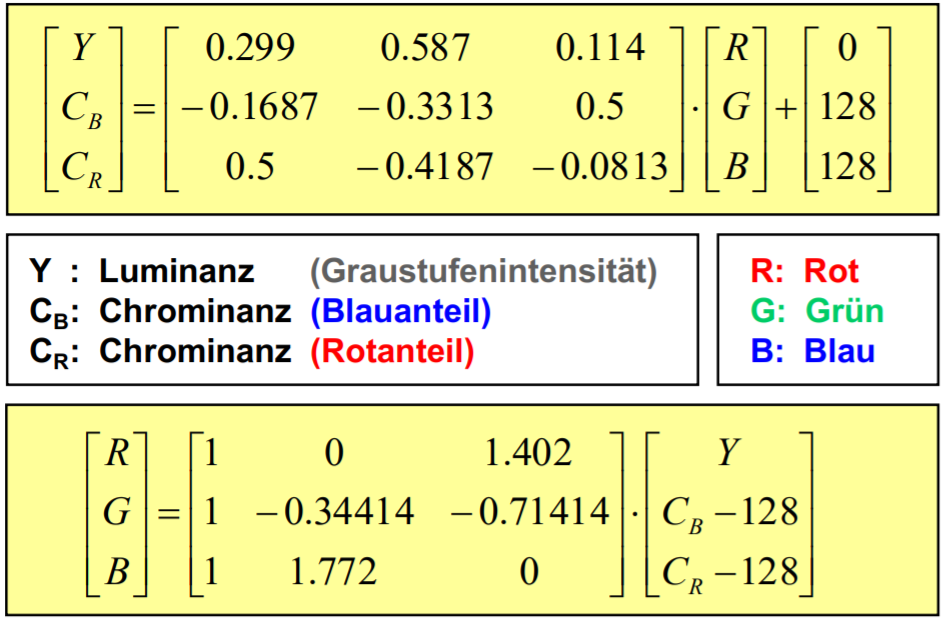
\includegraphics[width=1\linewidth]{images/lumchrom.png}
\end{center}

\subsubsection{Downsampling}

Bei Downsampling werden in beiden Chrominanz-Ebenen in der Horizontalen oder Vertikalen mehrere Pixel zusammengefasst. \\
\textbf{Beispiel: } 4:2:0, 4 bezeichnet hier die Breite des Referenzblocks, 2 bezeichnet wie viele Pixel nach dem Downsampling auf der ersten Zeile und 0 auf der zweiten Zeile vorliegen.
\begin{center}
    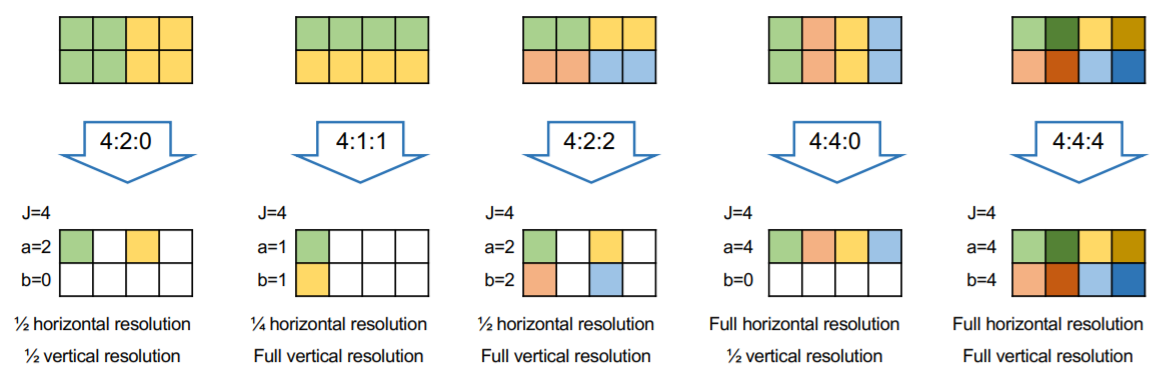
\includegraphics[width=1\linewidth]{images/downsampling.png}
\end{center}

\subsubsection{JPEG Blockverarbeitung}

\begin{center}
    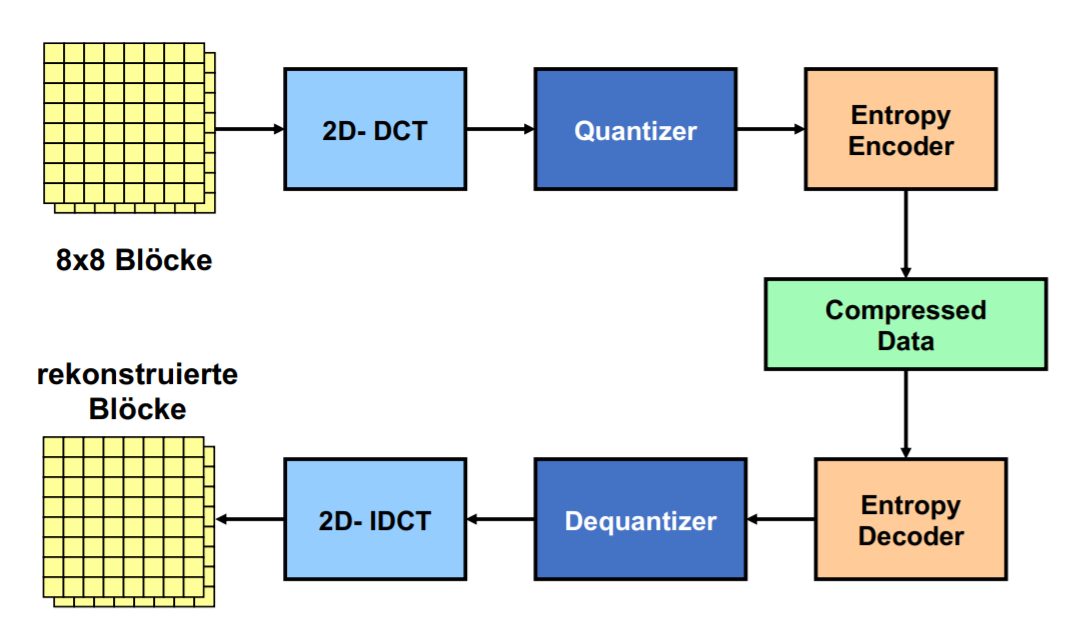
\includegraphics[width=1\linewidth]{images/blockverarbeitung.png}
\end{center}

\subsubsection{DCT Basisfunktion}

\begin{center}
    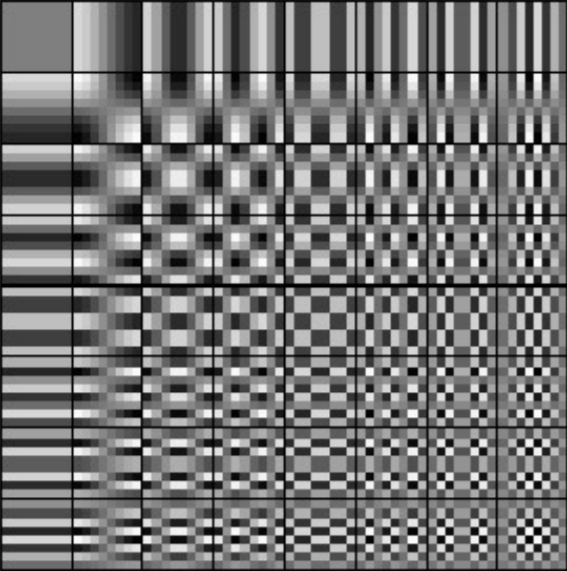
\includegraphics[width=0.6\linewidth]{images/dct.png}
\end{center}

\begin{center}
    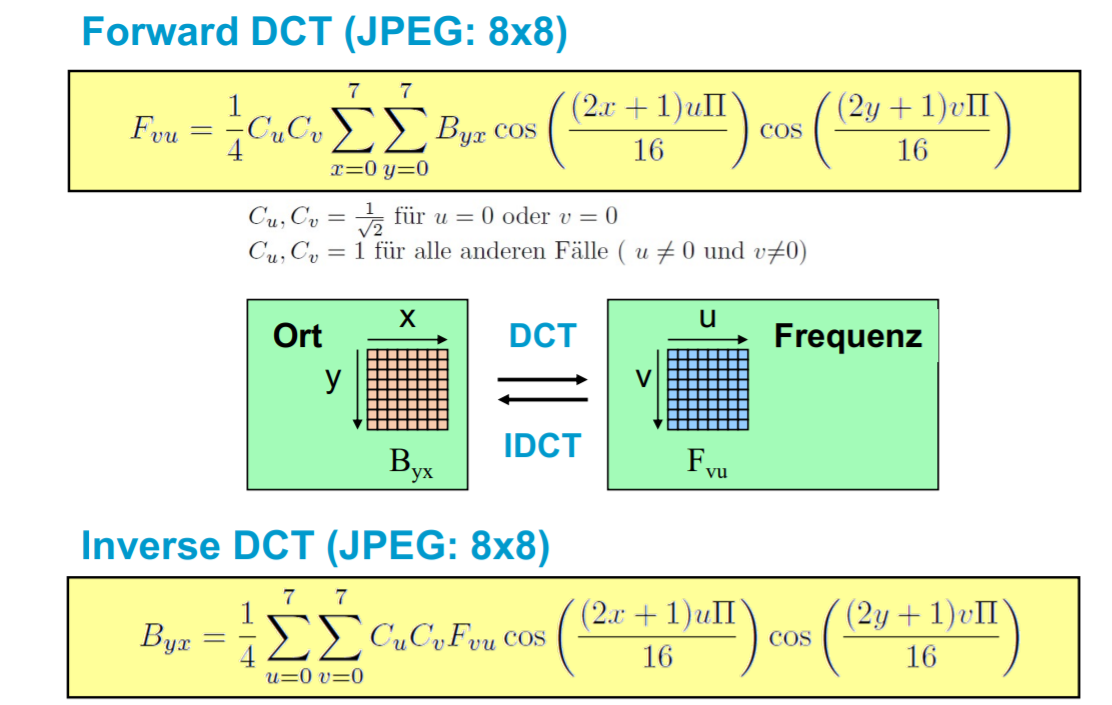
\includegraphics[width=1\linewidth]{images/dctfunction.png}
\end{center}

\begin{center}
    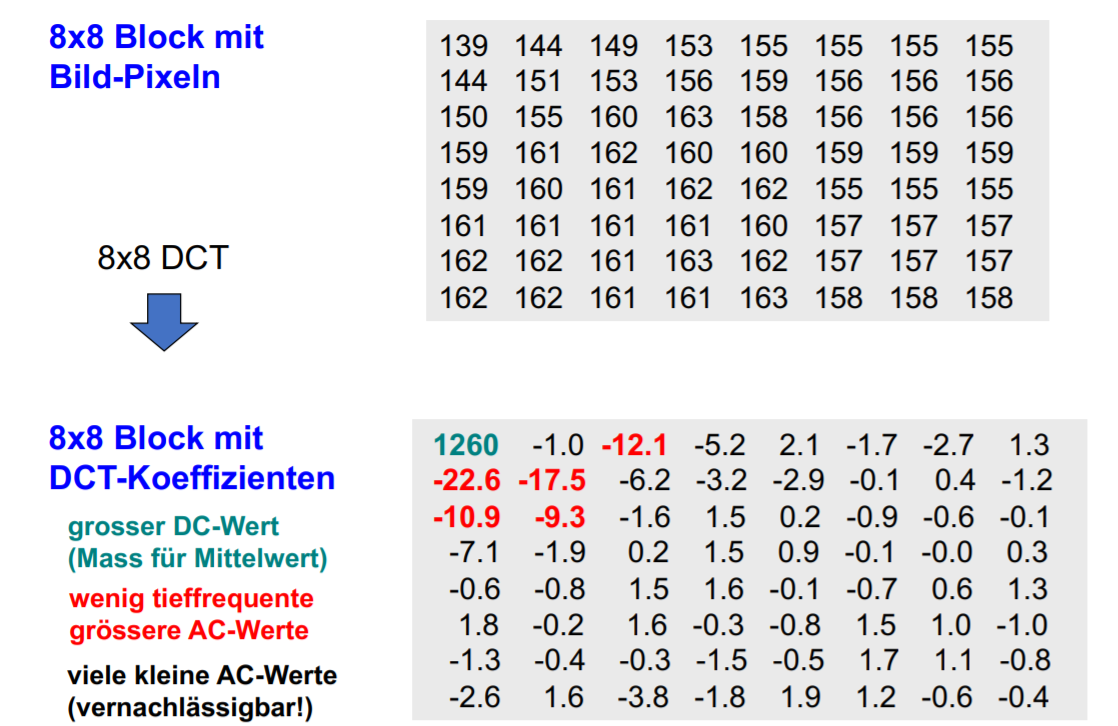
\includegraphics[width=1\linewidth]{images/dctblock.png}
\end{center}

\subsubsection{Quantisierung}%

\begin{center}
    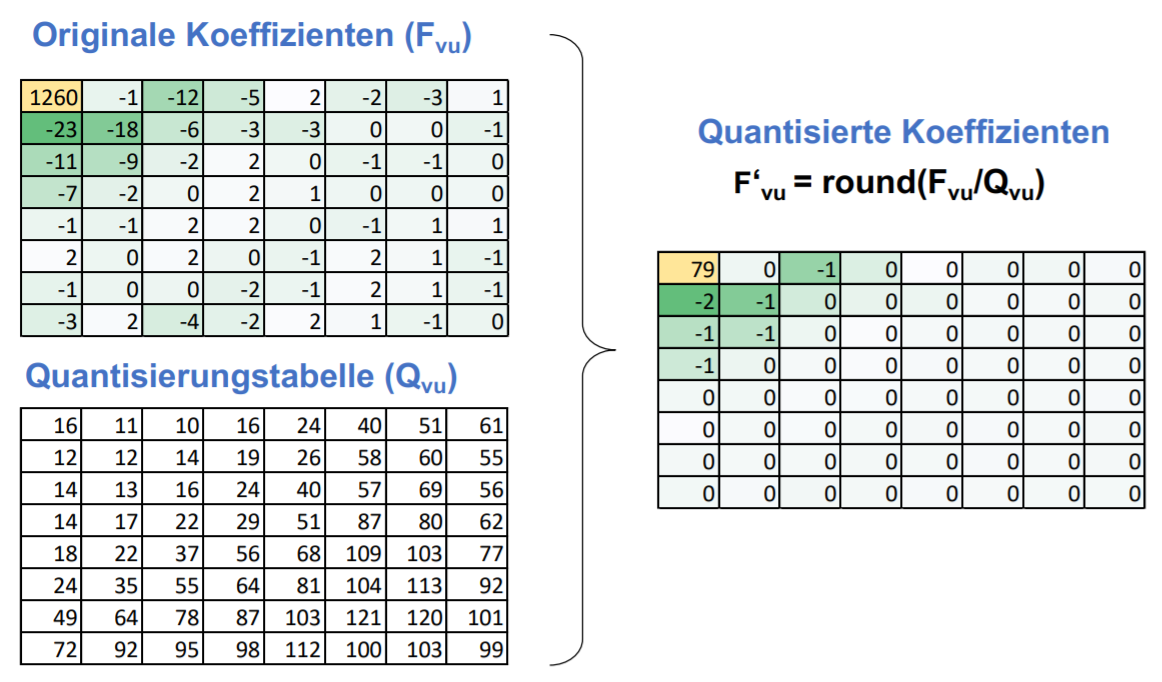
\includegraphics[width=1\linewidth]{images/quantisierung.png}
\end{center}

\subsubsection{Entropy Encoder}

\begin{center}
    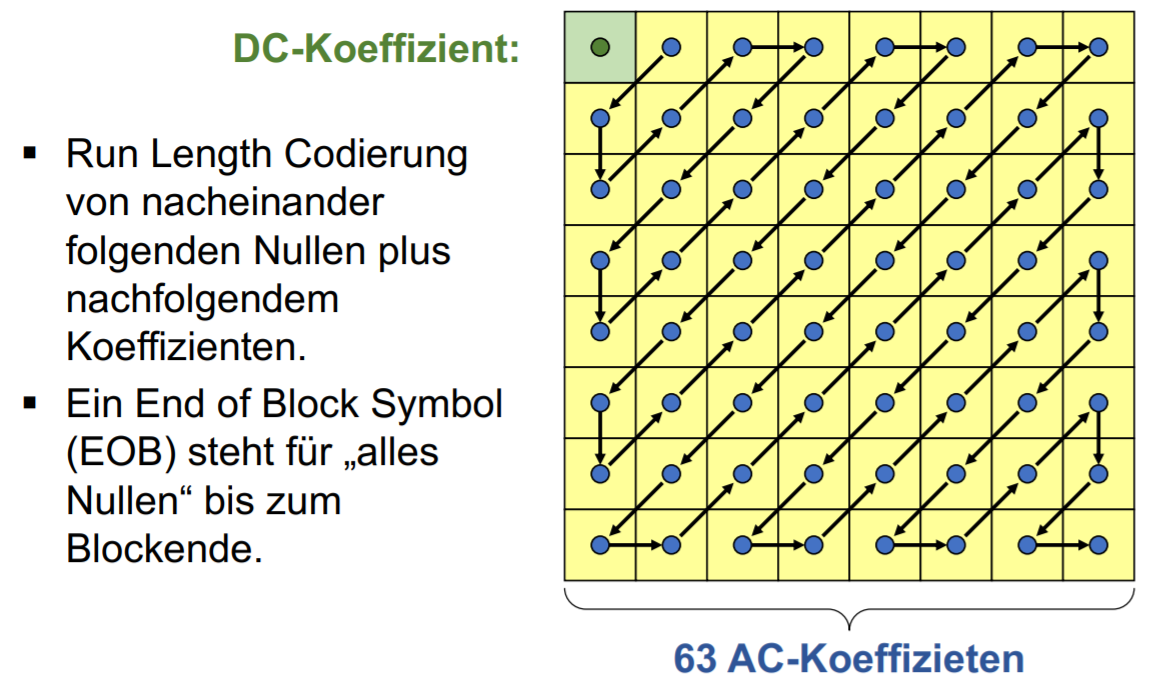
\includegraphics[width=1\linewidth]{images/entropy_encoding.png}
\end{center}

RLE: (DC Wert) (Anzahl Nullen, Koeffizient)...(EOB)

\subsubsection{Dequantisierung}%

\begin{center}
    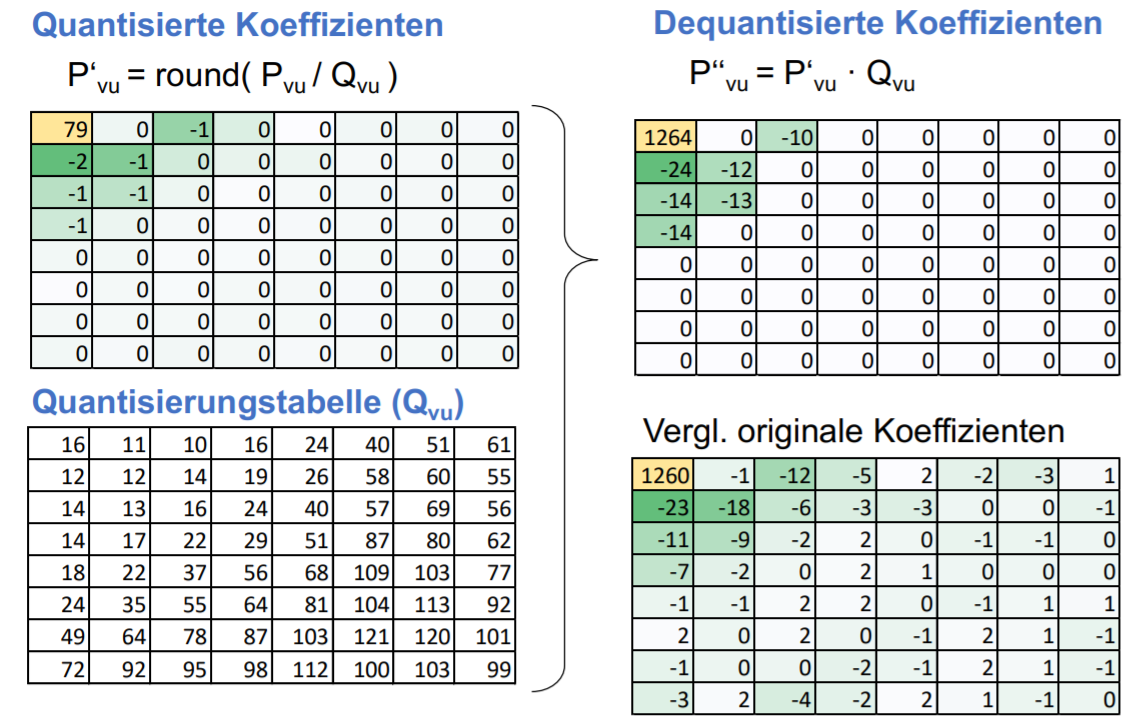
\includegraphics[width=1\linewidth]{images/dequantisierung.png}
\end{center}
